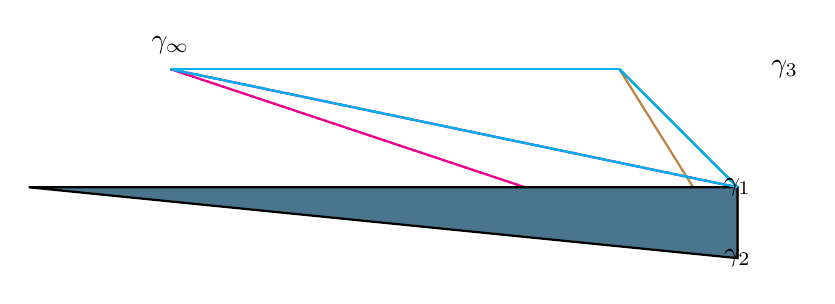
\begin{tikzpicture}[scale=0.3, thick]
	\begin{scope}[rotate=0]
		\coordinate (O) at (-9,-1);
		\coordinate (G) at (10,-1);
		\coordinate (B) at (15,-6);
		\coordinate (A) at (-15,-6);
		\coordinate (C) at (15,-9);
		
		\draw[red,dotted] (O) -- (C) node[midway,above,sloped]{};
		\draw[red,dotted] (C) -- (B) node[midway,right]{};
		\draw[red,dotted] (B) -- (O) node[midway,above,sloped]{};
		
		\draw[magenta] (O) -- (C) node[midway,above,sloped]{};
		\draw[magenta] (C) -- (B) node[midway,right]{};
		\draw[magenta] (B) -- (O) node[midway,above,sloped]{};
		
		\draw[brown] (G) -- (B) node[midway,right]{};
		\draw[brown] (B) -- (C) node[midway,below]{};
		\draw[brown] (C) -- (G) node[midway,left]{};
		
		\draw[cyan] (O) -- (G) node[midway,below]{};
		\draw[cyan] (G) -- (B) node[midway,right]{};
		\draw[cyan] (B) -- (O) node[midway,below]{};
		
		\filldraw[fill=cyan!50!black] (A) -- (B) -- (C) -- cycle;
		\draw[dashed,cyan] (O) -- (G) node[midway,below]{};
		\draw[dashed,cyan] (G) -- (B) node[midway,right]{};
		\draw[dashed,cyan] (B) -- (O) node[midway,below]{};
		
		\node at (-9,0) {$\gamma_\infty$};
		\node at (15,-6) {$\gamma_1$};
		\node at (15,-9) {$\gamma_2$};
		\node at (17,-1) {$\gamma_3$};
	\end{scope}
\end{tikzpicture}